% !TEX root = ../../Dissertation.tex

\begin{refsection}

\chapter[Small chromium oxide clusters]{Geometric, Electronic, and magnetic properties of Small Chromium oxide clusters} \label{CrxOy}


\definecolor{shadecolor}{gray}{0.85}
\begin{shaded}
\textbf{This chapter is based on the paper:}\\
Pham, L. N.; Claes, P.; Lievens, P.; Jiang, L.; Wende, T.; Asmis, K. R.; Nguyen, M. T.; Janssens, E. Geometric Structures and Magnetic Interactions in Small Chromium Oxide Clusters. \textit{J. Phys. Chem. C} \textit{2018}, 122, 27640-27647. \textit{Reprinted with permission from Journal of Physical Chemistry C. Copyright 2018. American Chemical Society.} \textcolor{blue}{\href{https://pubs.acs.org/doi/suppl/10.1021/acs.jpcc.8b10035/suppl_file/jp8b10035_si_002.pdf}{The Supporting Information is available online}}

\emph{My contribution to this work was theoretical calculations, data analysis, discussion, writing of the first draft and revision.}
\newpage
\end{shaded}


\section{Introduction}

Bulk chromium is an antiferromagnetic material at room temperature (its N\'{e}el temperature is about 308 K) and behaves paramagnetically at higher temperatures.\cite{Fawcett1988} The chromium atom has, in the ground state, six unpaired electrons in its 3\textit{d} and 4\textit{s} orbitals. In the smallest possible cluster of chromium atoms, the \ch{Cr2} dimer, the total magnetic moment is zero as a result of antiferromagnetic coupling of the local moments.\cite{bondybey1983, Riley1983, Zamudio2015} Interestingly, the \ch{Cr-Cr} bond length is significantly increased and the local moments at the two chromium sites couple ferromagnetically if one electron is removed resulting in a high-spin ground state ($^{12}\Sigma$) for \ch{Cr2+}.\cite{Zamudio2015} Triatomic and other small odd sized chromium clusters are subject to antiferromagnetic frustration.\cite{Janssens2007,Cheng1996} In a recent theoretical study, an energetic competition between low and high spin states (S = 1 and S = 6) was found in \ch{Cr4} as a result of the highly correlated electron behavior.\cite{Estrada-Cr4}


Magnetic interactions in pure chromium clusters can be altered by addition of oxygen atoms. Superexchange through bridging oxygen atoms induces a ferromagnetic coupling between the local moments on the two Cr atoms in \ch{Cr2O_n^{-/0}} (n = 1 -- 3). \cite{Tono2003,Tono2003B}  Further addition of oxygen reduces, and even quenches, total magnetic moments of the dichromium clusters (\ch{Cr2O_n}, n = 4 -- 14).\cite{Reddy2000Cr2On,GutsevCr2On} A similar observation was made for larger clusters; the local magnetic moments of chromium atoms are quenched in clusters with a high oxygen concentration, such as \ch{Cr4O10} and \ch{(CrO3)_n} (n = 1 -- 5).\cite{Li2012,Zhai2008} Such quenching happens because all chromium valence electrons are involved in chemical bonds with oxygen atoms. In suboxide clusters, such as \ch{Cr3O_n^{+/0}} (n = 0 -- 3), the magnetic interactions are controlled by the amount of oxygen. \cite{Janssens2007} Besides the composition (chromium to oxygen atomic ratio), also the precise geometry of the cluster is important for the magnetic interaction. It was, for example, found that \ch{Cr_nO2} (n = 2 -- 5) clusters of the same size but with a different geometric structure can have different magnetic properties and interactions. \cite{ pakiari2016, Shah2018} Similar findings were reported for iron oxide clusters. For example, different magnetic states were predicted as lowest energy configuration of the neutral \ch{Fe4O6}, although these isomers have similar geometries (T$_d$ versus slightly distorted T$_d$ symmetry), including a ferromagnetic state with a magnetic moment of 20 $\mu_B$, \cite{fe4o6-Ding} a ferrimagnetic 10 $\mu_B$ state, \cite{fe4o6-Kirilyuk} and most recently a singlet state ($^1$A$_2$, C$_{2v}$). \cite{Logemann2015, Erlebach14} Therefore, it is important to identify the geometry of clusters produced in the experiment before assessing their magnetic ground state configurations. The cluster geometry can be accurately obtained from infrared photodissociation (\acrshort{irpd}) spectroscopy experiments on cluster-rare gas atom complexes. The detachment of the rare gas atoms is detected mass spectrometrically and signals resonant absorption of infrared photons. This spectroscopic technique, in combination with density functional theory (\acrshort{dft}) calculations, has been proven a powerful technique to identify the geometries of small metal oxide clusters. \cite{Janssens2001, Logemann2015, Sant2008, Mathias03, Asmis07, Dijk2014} 






To fully understand the interplay between chemical compositions, geometric arrangements, and magnetic properties of small chromium oxide clusters, we synthesized a series of cationic \ch{Cr_mO_n+} (m =  2, 3, 4; n $\leq$ m) clusters and studied them by a combination of infrared spectroscopy and quantum chemical calculations. Several quantum chemical methods were employed to locate ground-state and low-lying structures of the synthesized clusters. The magnetic interactions between and/or among local sites were studied. The evolution of magnetic moments through chemical control is discussed. 

\section{Experimental Methods}

The experiments were carried out using a molecular beam setup consisting of a cluster source, an ion guide, a mass filter, an ion trap, and a time-of-flight mass spectrometer. \cite{Daniel2009} This setup was temporarily installed at the Free Electron Laser for Infrared eXperiments (FELIX) facility (The Netherlands).\cite{Oepts1995} The 2nd harmonic of a Nd:YAG laser is focused on a metallic Cr plate and creates a plasma, which is entrained in a pulse of 1\% \ch{O2} seeded in He carrier gas and expanded through a clustering channel. The chromium-oxide cluster beam is collimated and thermalized to room temperature by collisions with Ar atoms in a radio frequency (RF) decapole ion guide and mass-selected by a quadrupole mass filter. Mass-selected cationic clusters are accumulated in a ring electrode ion trap. To allow for continuous ion loading, ion thermalization, and cluster-rare gas (He, Ne) complex formation, the trap is continuously filled with a buffer gas of either pure He (for \ch{Cr3O+} and \ch{Cr3O2+}) or a mixture of 0.125\% Ne in He (for \ch{Cr2O2+}, \ch{Cr3O3+}, and \ch{Cr4O4+}) at ion trap temperatures in the range of 20 -- 35 K. After filling the trap for 98 ms, all ions are extracted and focused both temporally and spatially into the center of the extraction region of an orthogonally mounted linear time-of-flight (TOF) mass spectrometer. Here, the ion packet can be irradiated with the \acrshort{ir} laser pulse. The absorption of a few and often only a single \acrshort{ir} photon(s) by the weakly bound cluster-rare gas ionic complex is sufficient for vibrational predissociation and loss of the rare gas messenger. Scanning the wavelength of the excitation laser light provides the \acrshort{irpd} spectra, which are obtained in the difference mode of operation (laser on-laser off) and recorded by monitoring all ion intensities simultaneously. The infrared free electron laser FELIX is operated in the 400 -- 750 cm$^{-1}$ spectral range at a repetition rate of 5 Hz, a bandwidth of 0.2\% root-mean-square of the central wavelength and an average pulse energy of 10 mJ.

\section{Computational Methods}

The CALYPSO\cite{CALYPSO} tool was used to generate large numbers of initial structures at relatively low computational levels (B3LYP/3-21G and BP86/3-21G). The generated low-lying energetic structures were subsequently reoptimized with the larger cc-pVTZ basis set. \cite{basis-augM, basis-ccO} Different spin multiplicities were tested for all structural isomers. Various density functionals (B3LYP, \cite{lyp, b3lyp2, b3} B3P86, \cite{b3,p86} B3PW91, \cite{b3} BP86, \cite{b3lyp2, p86} TPSS, \cite{tpss} TPSSh, and M06L \cite{m06l}) have been tested to ensure reliability of the obtained results. In addition, for \ch{Cr2O2+} the restricted active space followed by second-order perturbation treatment (\acrshort{rasscf}/\acrshort{raspt2}) and coupled cluster (\acrshort{ccsd}(T)-F12) methods have been used as benchmark for the \acrshort{dft} calculations. More details about these computational processes are provided in the \href{https://pubs.acs.org/doi/suppl/10.1021/acs.jpcc.8b10035/suppl_file/jp8b10035_si_002.pdf}{\textcolor{blue}{Supporting Information}} (available online). Throughout the calculation process, the TPSS functional appears to be excellent in vibrational simulations of the obtained clusters in comparison to the other used functionals; therefore the simulated spectra from this functional are used as the basis for 4 out of 5 spectral assignments in this work. The B3P86 functional was used for \ch{Cr2O2+}, since the \acrshort{ir} spectrum of its $^8$B$_{1u}$ state could not be assessed at the TPSS level (see the \href{https://pubs.acs.org/doi/suppl/10.1021/acs.jpcc.8b10035/suppl_file/jp8b10035_si_002.pdf}{\textcolor{blue}{SI}} for details). \acrshort{dft} energies were corrected for zero point energies (\acrshort{zpe}s) at corresponding levels of theory, unless otherwise stated. The harmonic vibrational frequencies of the ground and first excited states were analytically obtained after \acrshort{dft} optimizations. If not explicitly specified in the text, harmonic vibrational frequencies were calculated with the Gaussian 09 program.\cite{g09} The empirical dispersion correction GD3 \cite{GD3} (for supported functionals) for optimizations and spectral simulations was taken into account.

  

\section{Results and Discussion}


\subsection{Structural Assignments} 



Starting from the simplest synthesized cluster \ch{Cr2O2+}, two clear bands around 610 and 720 cm$^{-1}$ were observed from the experimental \acrshort{irpd} spectrum of the \ch{Cr2O2+}$\boldsymbol{\cdot}$Ne complex. The ground, first excited states and other low-lying ones of \ch{Cr2O2+} are listed in Table \href{https://pubs.acs.org/doi/suppl/10.1021/acs.jpcc.8b10035/suppl_file/jp8b10035_si_002.pdf}{\textcolor{blue}{S1}} of the \href{https://pubs.acs.org/doi/suppl/10.1021/acs.jpcc.8b10035/suppl_file/jp8b10035_si_002.pdf}{\textcolor{blue}{SI}}. At all considered levels of theory the $^8$B$_{1g}$ and $^8$B$_{1u}$ states are much lower in energy, so we just focus on these two states. Comparing the geometrical structures of the $^8$B$_{1g}$ ground and the $^8$B$_{1u}$ excited states, small differences are found. The \ch{Cr-O} bond is 0.01 \AA\space longer when \ch{Cr2O2+} is stimulated from the $^8$B$_{1g}$ ground state to the $^8$B$_{1u}$ first excited state. The bonding angles $\widehat{OCrO}$ and $\widehat{CrOCr}$ also stretch and bend, respectively, 5 degrees in comparison to the ones of the ground state. In terms of electronic structures, these two states differentiate from each other in the occupation of electrons in b$_{1g}$ and b$_{1u}$ orbitals. The leading configurations of these different electronic states are given in Table \href{https://pubs.acs.org/doi/suppl/10.1021/acs.jpcc.8b10035/suppl_file/jp8b10035_si_002.pdf}{\textcolor{blue}{S2}} of the \href{https://pubs.acs.org/doi/suppl/10.1021/acs.jpcc.8b10035/suppl_file/jp8b10035_si_002.pdf}{\textcolor{blue}{SI}}. 




The difference in energy between the ground state $^8$B$_{1g}$ and first excited state $^8$B$_{1u}$ at the \acrshort{raspt2} level is 0.38 eV. Assuming Maxwell-Boltzmann statistics, occupancy of an excited state at +0.38 eV would be small. However, besides uncertainty on the calculated relative energy of the excited state, also the attachment of messenger rare gases may affect the energy differences between isomers. Because of shortcomings of the implementation of the \acrshort{raspt2} calculational technique, the effect of rare gas messenger atoms on the excited states of \ch{Cr2O2+} cannot be examined precisely. Taking into account the computational uncertainty of \acrshort{raspt2} and other quantum chemical methods, the differences in geometrical structures of the ground and first excited states are insignificant, and it is well possible that both the ground and first excited state are populated in the experiment. 




The experimental \acrshort{irpd} and simulated \acrshort{ir} spectra of the \ch{Cr2O2+} cluster are presented in Figure \ref{fig:Cr2O2}. Although the TPSS functional is used for simulating the vibrational spectra of most clusters studied in this work, the simulated \acrshort{ir} spectrum of excited state \ch{^8B_{1u}} could not be accessed at this level; therefore, the simulated spectra of these two states at the B3P86 level are used in Figure \ref{fig:Cr2O2}b. The simulated \acrshort{ir} spectrum in Figure \ref{fig:Cr2O2}b is consistent with those obtained for the same isomer using other \acrshort{dft} functionals (TPSSH, B3PW91, B3P86, B3LYP, M06L, and BP86) (see Figure \href{https://pubs.acs.org/doi/suppl/10.1021/acs.jpcc.8b10035/suppl_file/jp8b10035_si_002.pdf}{\textcolor{blue}{S9}} of the \href{https://pubs.acs.org/doi/suppl/10.1021/acs.jpcc.8b10035/suppl_file/jp8b10035_si_002.pdf}{\textcolor{blue}{SI}}). Note that the interaction of the cationic chromium oxide clusters with the rare gas messenger atoms (Ne and He) does not significantly affect the simulated \acrshort{ir} spectra (see Figure \href{https://pubs.acs.org/doi/suppl/10.1021/acs.jpcc.8b10035/suppl_file/jp8b10035_si_002.pdf}{\textcolor{blue}{S2}} of the \href{https://pubs.acs.org/doi/suppl/10.1021/acs.jpcc.8b10035/suppl_file/jp8b10035_si_002.pdf}{\textcolor{blue}{SI}}). 

\begin{figure}[htb!]
	\centering
	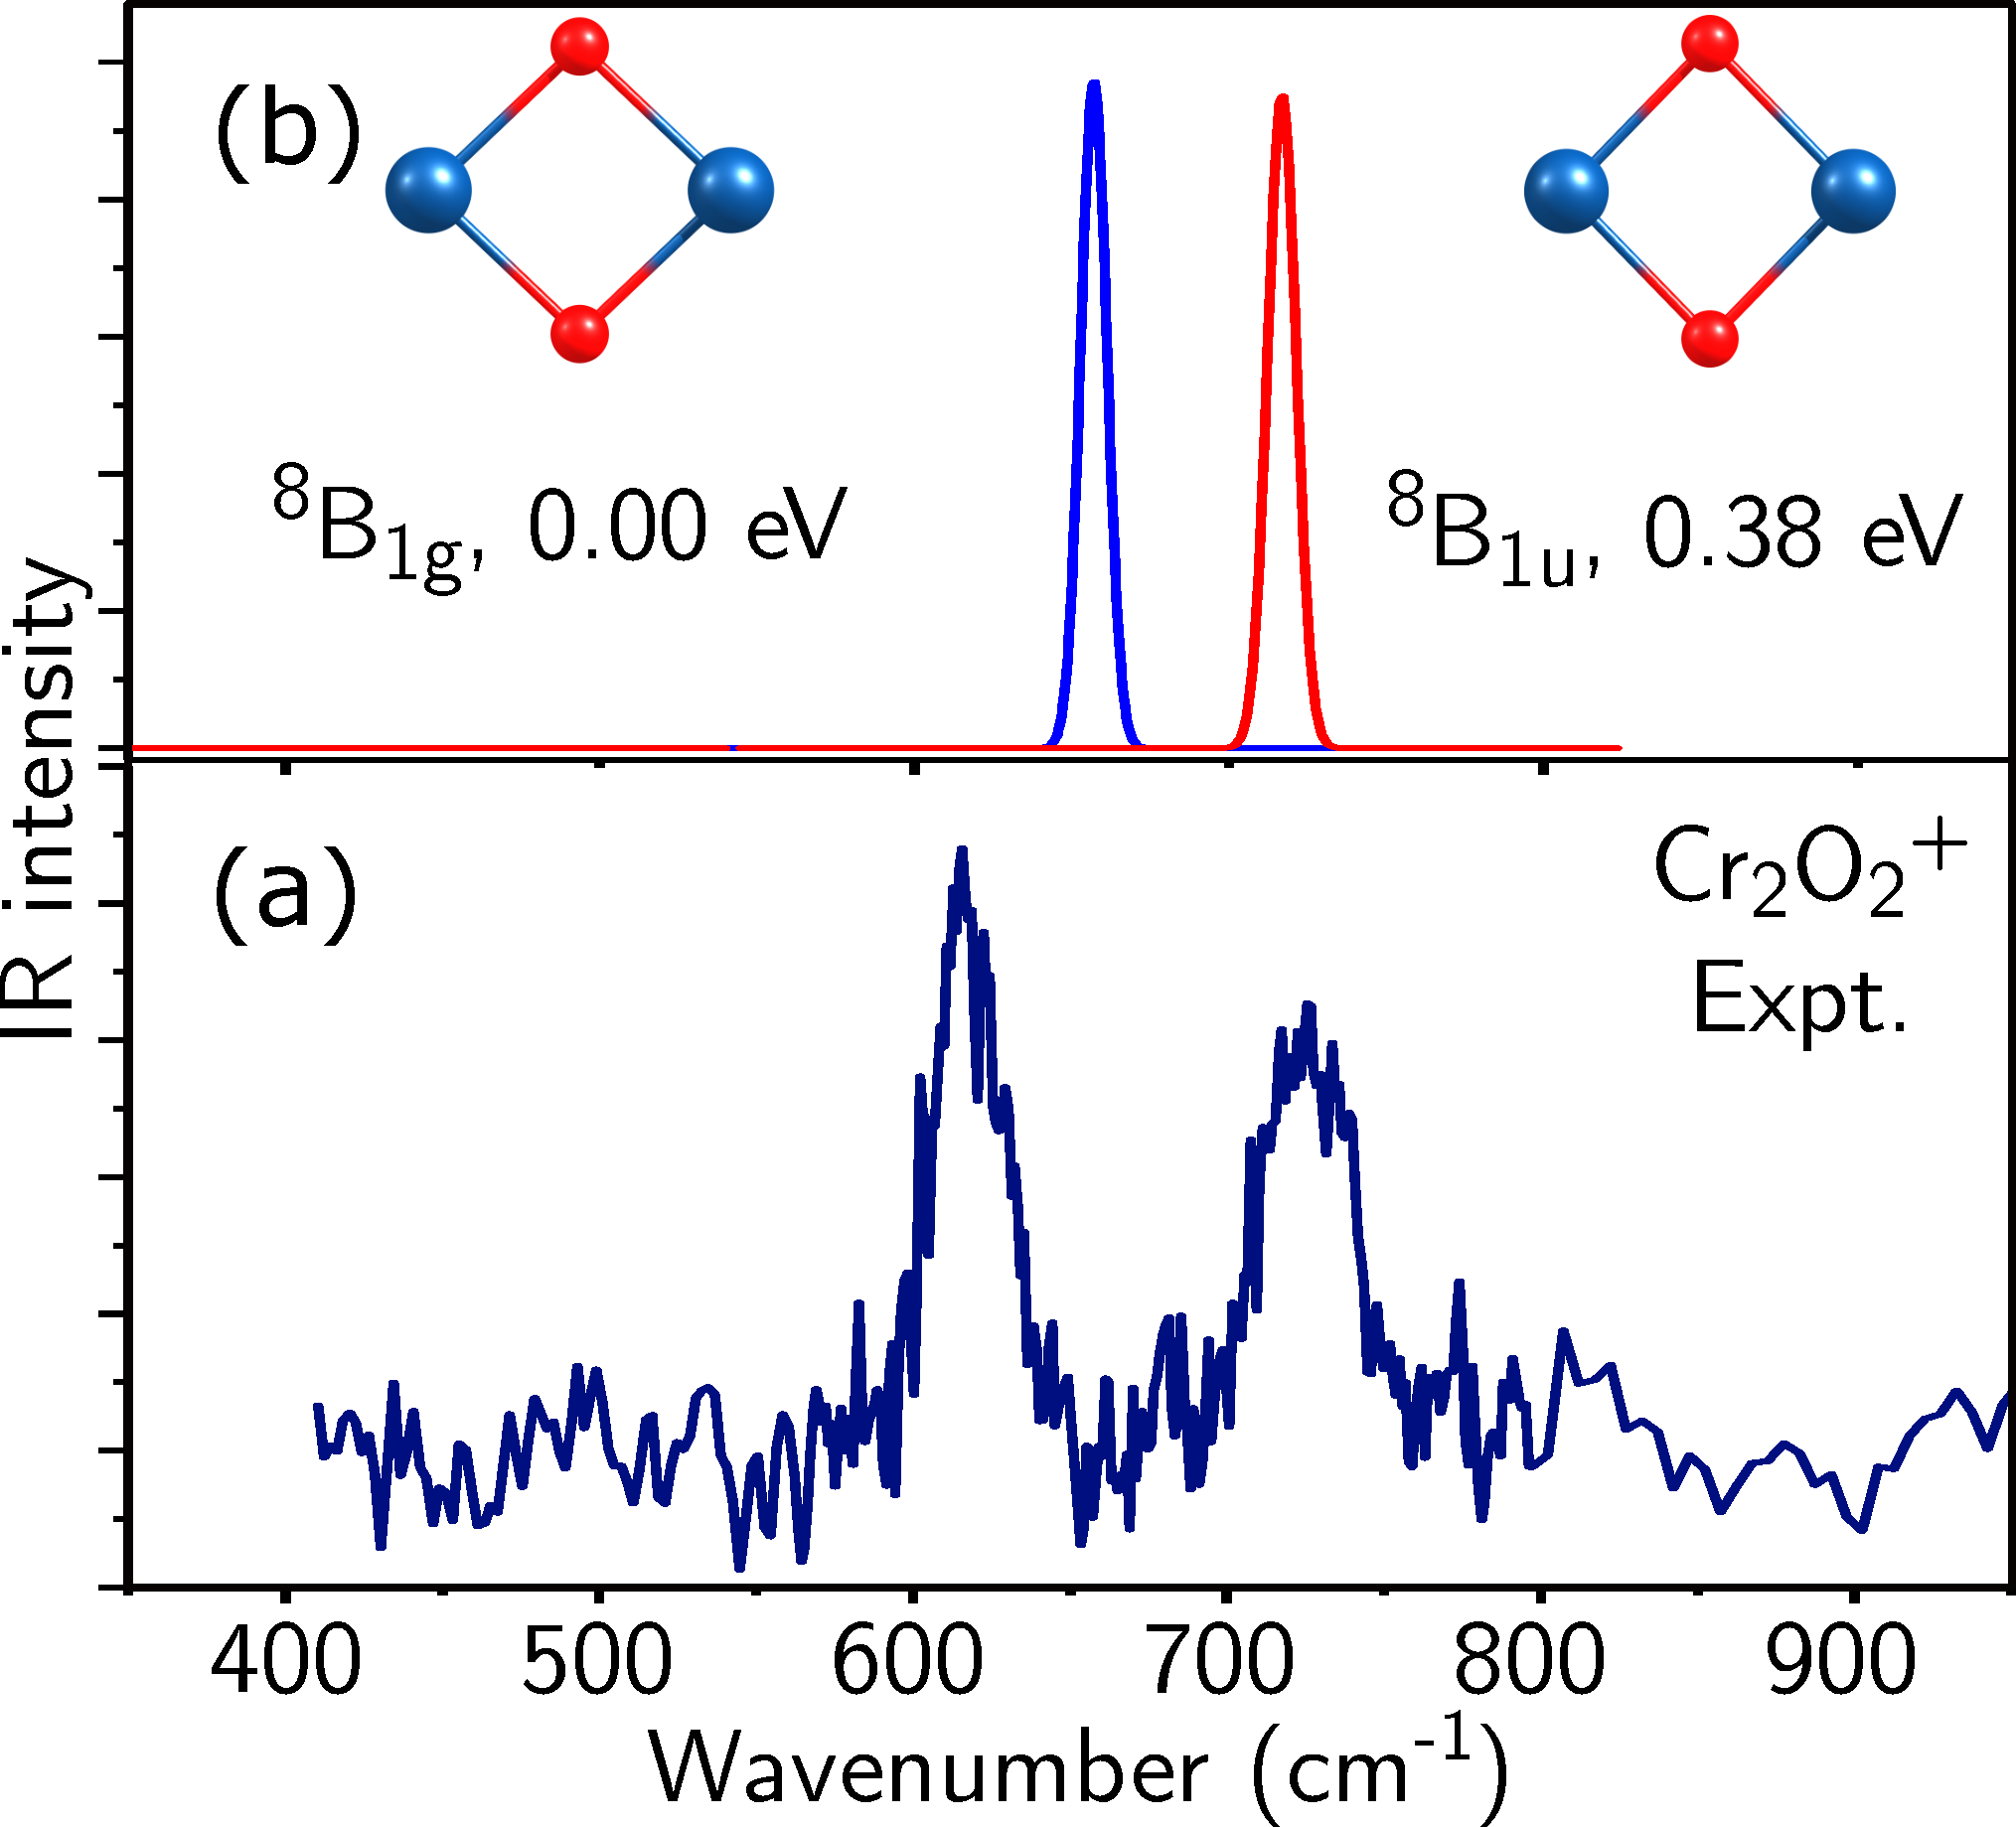
\includegraphics[width=0.4\textwidth]{Cr2O2}
	\caption{(a) Experimental \acrshort{irpd} spectra and (b) simulated harmonic \acrshort{ir} spectra of \ch{Cr2O2+}. The simulated spectrum of the $^8$B$_{1g}$ ground state is presented by the blue line, the spectrum of the $^8$B$_{1u}$ excited state by the red line. The geometries of the lowest-lying states are shown as insets.}
	\label{fig:Cr2O2}
\end{figure}



The simulated \acrshort{ir} spectrum of the ground state ($^8$B$_{1g}$) shows a single peak at around 630 cm$^{-1}$, which can only explain one of two experimental bands (Figure \ref{fig:Cr2O2}a). The first excited $^8$B$_{1u}$ state's simulated spectrum has a vibrational mode at around 700 cm$^{-1}$, 70 cm$^{-1}$ above that of the $^8$B$_{1g}$ ground state (see Figure \ref{fig:Cr2O2}b). Their separation agrees reasonably well with the observed band separation of 90 cm$^{-1}$ in the experimental spectrum. Therefore, both the $^8$B$_{1g}$ ground state and the $^8$B$_{1u}$ first excited state are proposed to be populated in the experiment. A similar observation has been made for \ch{Cr2O2^{-/0}}. \cite{nhanCr2O2} 




Figure \ref{fig:Cr3Ox} presents experimental and simulated spectra of the \ch{Cr3O_n+} (n = 1 -- 3) series. The \acrshort{ir} spectrum of \ch{Cr3O+}$\boldsymbol{\cdot}$\ch{He2} has a rather low signal-to-noise ratio, but shows a pronounced peak at 700 cm$^{-1}$ (see Figure \ref{fig:Cr3Ox}c). The lowest state is found to be $^6$A' for a propeller-like isomer within the C$_s$ symmetry. A D$_{3h}$ isomer with a high spin $^{16}$A$'$ electronic state is identified as the first excited state. The predicted \acrshort{ir} spectrum of the $^6$A$'$ ground state is in agreement with the experimental \acrshort{irpd} spectrum, i.e. the \acrshort{ir}-active peak observed at 700 cm$^{-1}$ is reproduced at 707 cm$^{-1}$. The \acrshort{ir} spectrum of the first excited state does not match the experimental spectrum, because its intense mode is about 150 cm$^{-1}$ red-shifted from the experimental feature.


\begin{figure}[htb!]
	\centering
	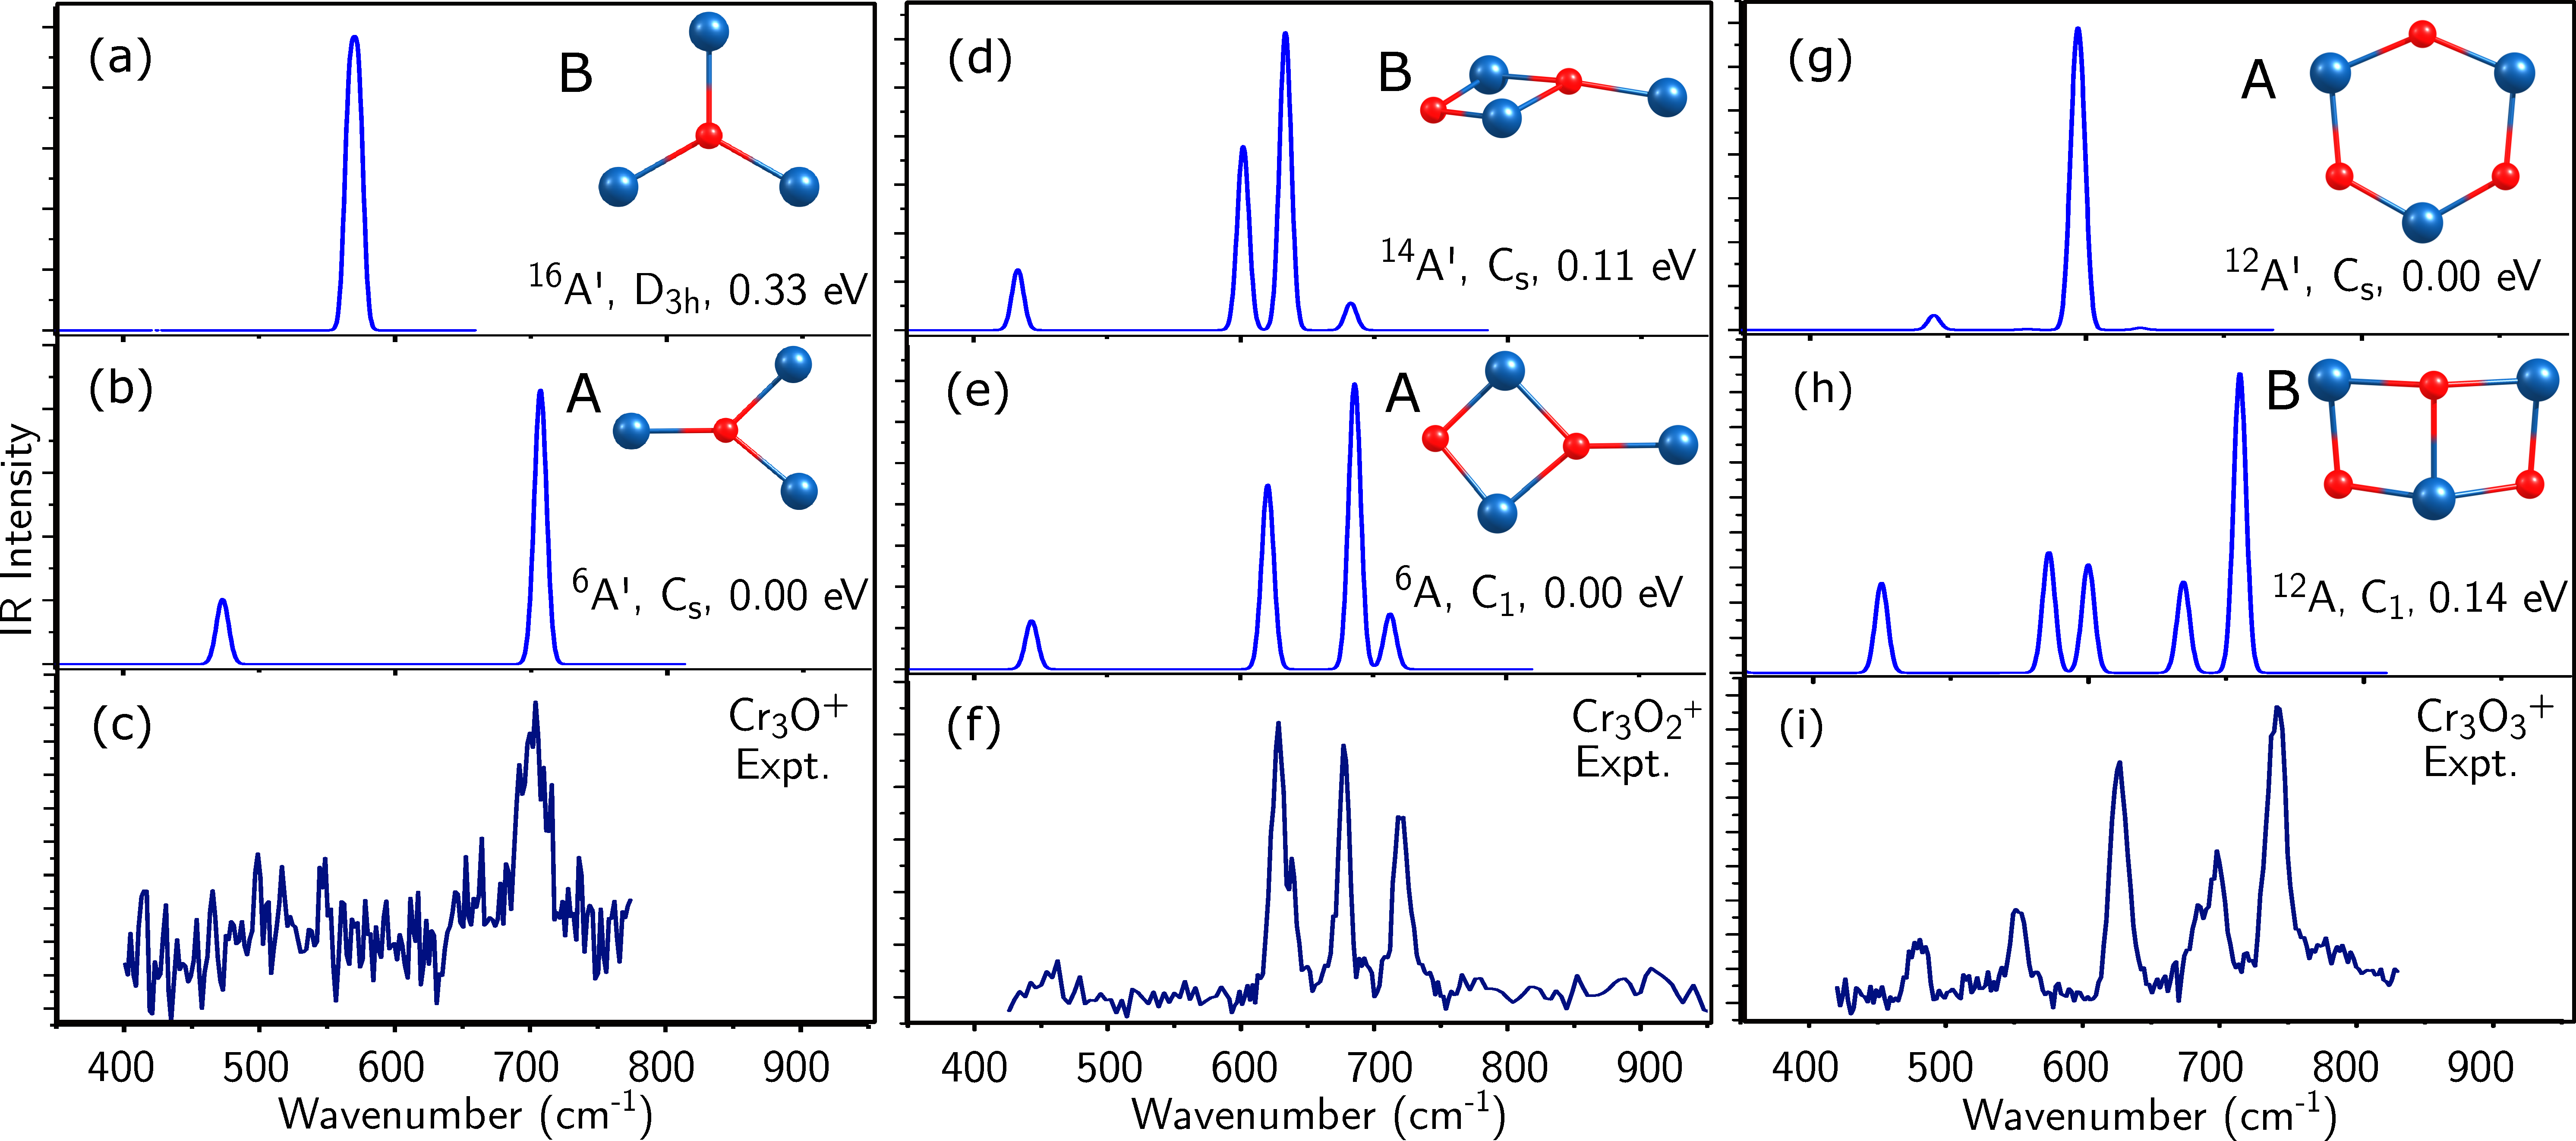
\includegraphics[width=\textwidth]{Cr3Ox}
	\caption{Experimental \acrshort{irpd} spectra and simulated harmonic \acrshort{ir} spectra of \ch{Cr3O+}, \ch{Cr3O2+}, and \ch{Cr3O3+}. The geometries of lowest-lying states for each cluster are shown as insets.}
	\label{fig:Cr3Ox}
\end{figure}



The \acrshort{irpd} spectrum of \ch{Cr3O2+}, measured on the \ch{Cr3O2+}$\boldsymbol{\cdot}$He complex, has three clear bands at 630, 680, and  725 cm$^{-1}$. The simulated \acrshort{ir} spectra of the sextet ground and a 14-et first excited state (see Figure \ref{fig:Cr3Ox}d and \ref{fig:Cr3Ox}e) were used to determine the experimentally populated structure of \ch{Cr3O2+}. For the $^6$A state, the TPSS method reproduces the three main experimental infrared active vibrations. Simulated spectra of these isomers using other \acrshort{dft} functionals are similar and can be found in the \href{https://pubs.acs.org/doi/suppl/10.1021/acs.jpcc.8b10035/suppl_file/jp8b10035_si_002.pdf}{\textcolor{blue}{SI}} (Figure \href{https://pubs.acs.org/doi/suppl/10.1021/acs.jpcc.8b10035/suppl_file/jp8b10035_si_002.pdf}{\textcolor{blue}{S11}}). We note that calculated harmonic \acrshort{ir} spectra are typically reliable to reproduce the number and the frequencies of the vibrational modes that are seen experimental, but are less accurate for predicting the relative intensities of those modes. The main reasons for this are the multiple photon aspect and the statistical dissociation of the cluster-rare gas complexes in the experiment, which are not included in the computations. A detailed discussion of the consequences of those effects can be found in ref \citenum{Calvo}. So we conclude that the sextet state is likely the isomer that is observed in the experiment. However, the first excited state $^{14}$A$'$ is quite close to the ground state in terms of energy (+0.11 eV at the TPSS level), and its simulated spectrum is similar to the one of the $^6$A state. Therefore, both isomers may coexist in the experiment.   




For \ch{Cr3O3+} two isomers with a high spin 12-tet (noted as A and B in Figure \ref{fig:Cr3Ox} parts g and h, respectively) are energetically competitive. Although the calculated relative energy of isomer B (+0.14 eV) is slightly higher than that of isomer A, its simulated \acrshort{ir} spectrum agrees much better with the experiment performed on the \ch{Cr3O3+}$\boldsymbol{\cdot}$Ne complex with regard to the frequency of the modes and the number of peaks. We, therefore, assign the spectrum to isomer B. Note that the relative energy difference is comparable to the accuracy of the computational method. As reported in Table the \href{https://pubs.acs.org/doi/suppl/10.1021/acs.jpcc.8b10035/suppl_file/jp8b10035_si_002.pdf}{\textcolor{blue}{S6}} of the \href{https://pubs.acs.org/doi/suppl/10.1021/acs.jpcc.8b10035/suppl_file/jp8b10035_si_002.pdf}{\textcolor{blue}{SI}}, different hybrid and metaGGA functionals either predict isomer A (TPSS, B3LYP, B3PW91, TPSSH) or isomer B (M06L, B3P86) as most stable isomer with a maximal energy difference of 0.17 eV.




The \acrshort{irpd} spectrum of \ch{Cr4O4^+} (see Figure \ref{fig:Cr4O4}) shows several vibrational bands, which are grouped in three ranges: 550-600 cm$^{-1}$, 650-710 cm$^{-1}$ and 750-790 cm$^{-1}$. In the computational study, many different local minima were obtained for \ch{Cr4O4+}. Two structural motifs were found to be more stable: a cage-like structure (isomer A) and a ring-like structure (isomer B). Two most stable isomers of \ch{Cr4O4+}, their lowest energy electronic states, and corresponding simulated \acrshort{ir} spectra are visualized in Figure \ref{fig:Cr4O4}. The simulated \acrshort{ir} spectrum of isomer A in the octet state is in substantially better agreement with the experiment performed on the \ch{Cr4O4+}$\boldsymbol{\cdot}$Ne complex, than that of isomer B. The only discrepancy is a redshift of the simulated spectrum by 40 cm$^{-1}$,  particularly for the intense bands in the 670-760 cm$^{-1}$ range. However, with the B3LYP, B3PW91 and B3P86 functional (see Figure \href{https://pubs.acs.org/doi/suppl/10.1021/acs.jpcc.8b10035/suppl_file/jp8b10035_si_002.pdf}{\textcolor{blue}{S13}} in the \href{https://pubs.acs.org/doi/suppl/10.1021/acs.jpcc.8b10035/suppl_file/jp8b10035_si_002.pdf}{\textcolor{blue}{SI}}), the redshift for these bands is much smaller (< 10 cm$^{-1}$). The \acrshort{ir} spectrum of the cyclic isomer B only predicts two \acrshort{ir}-active bands and cannot explain the more complex spectrum observed in the experiment.


\begin{figure}[htb!]
	\centering
	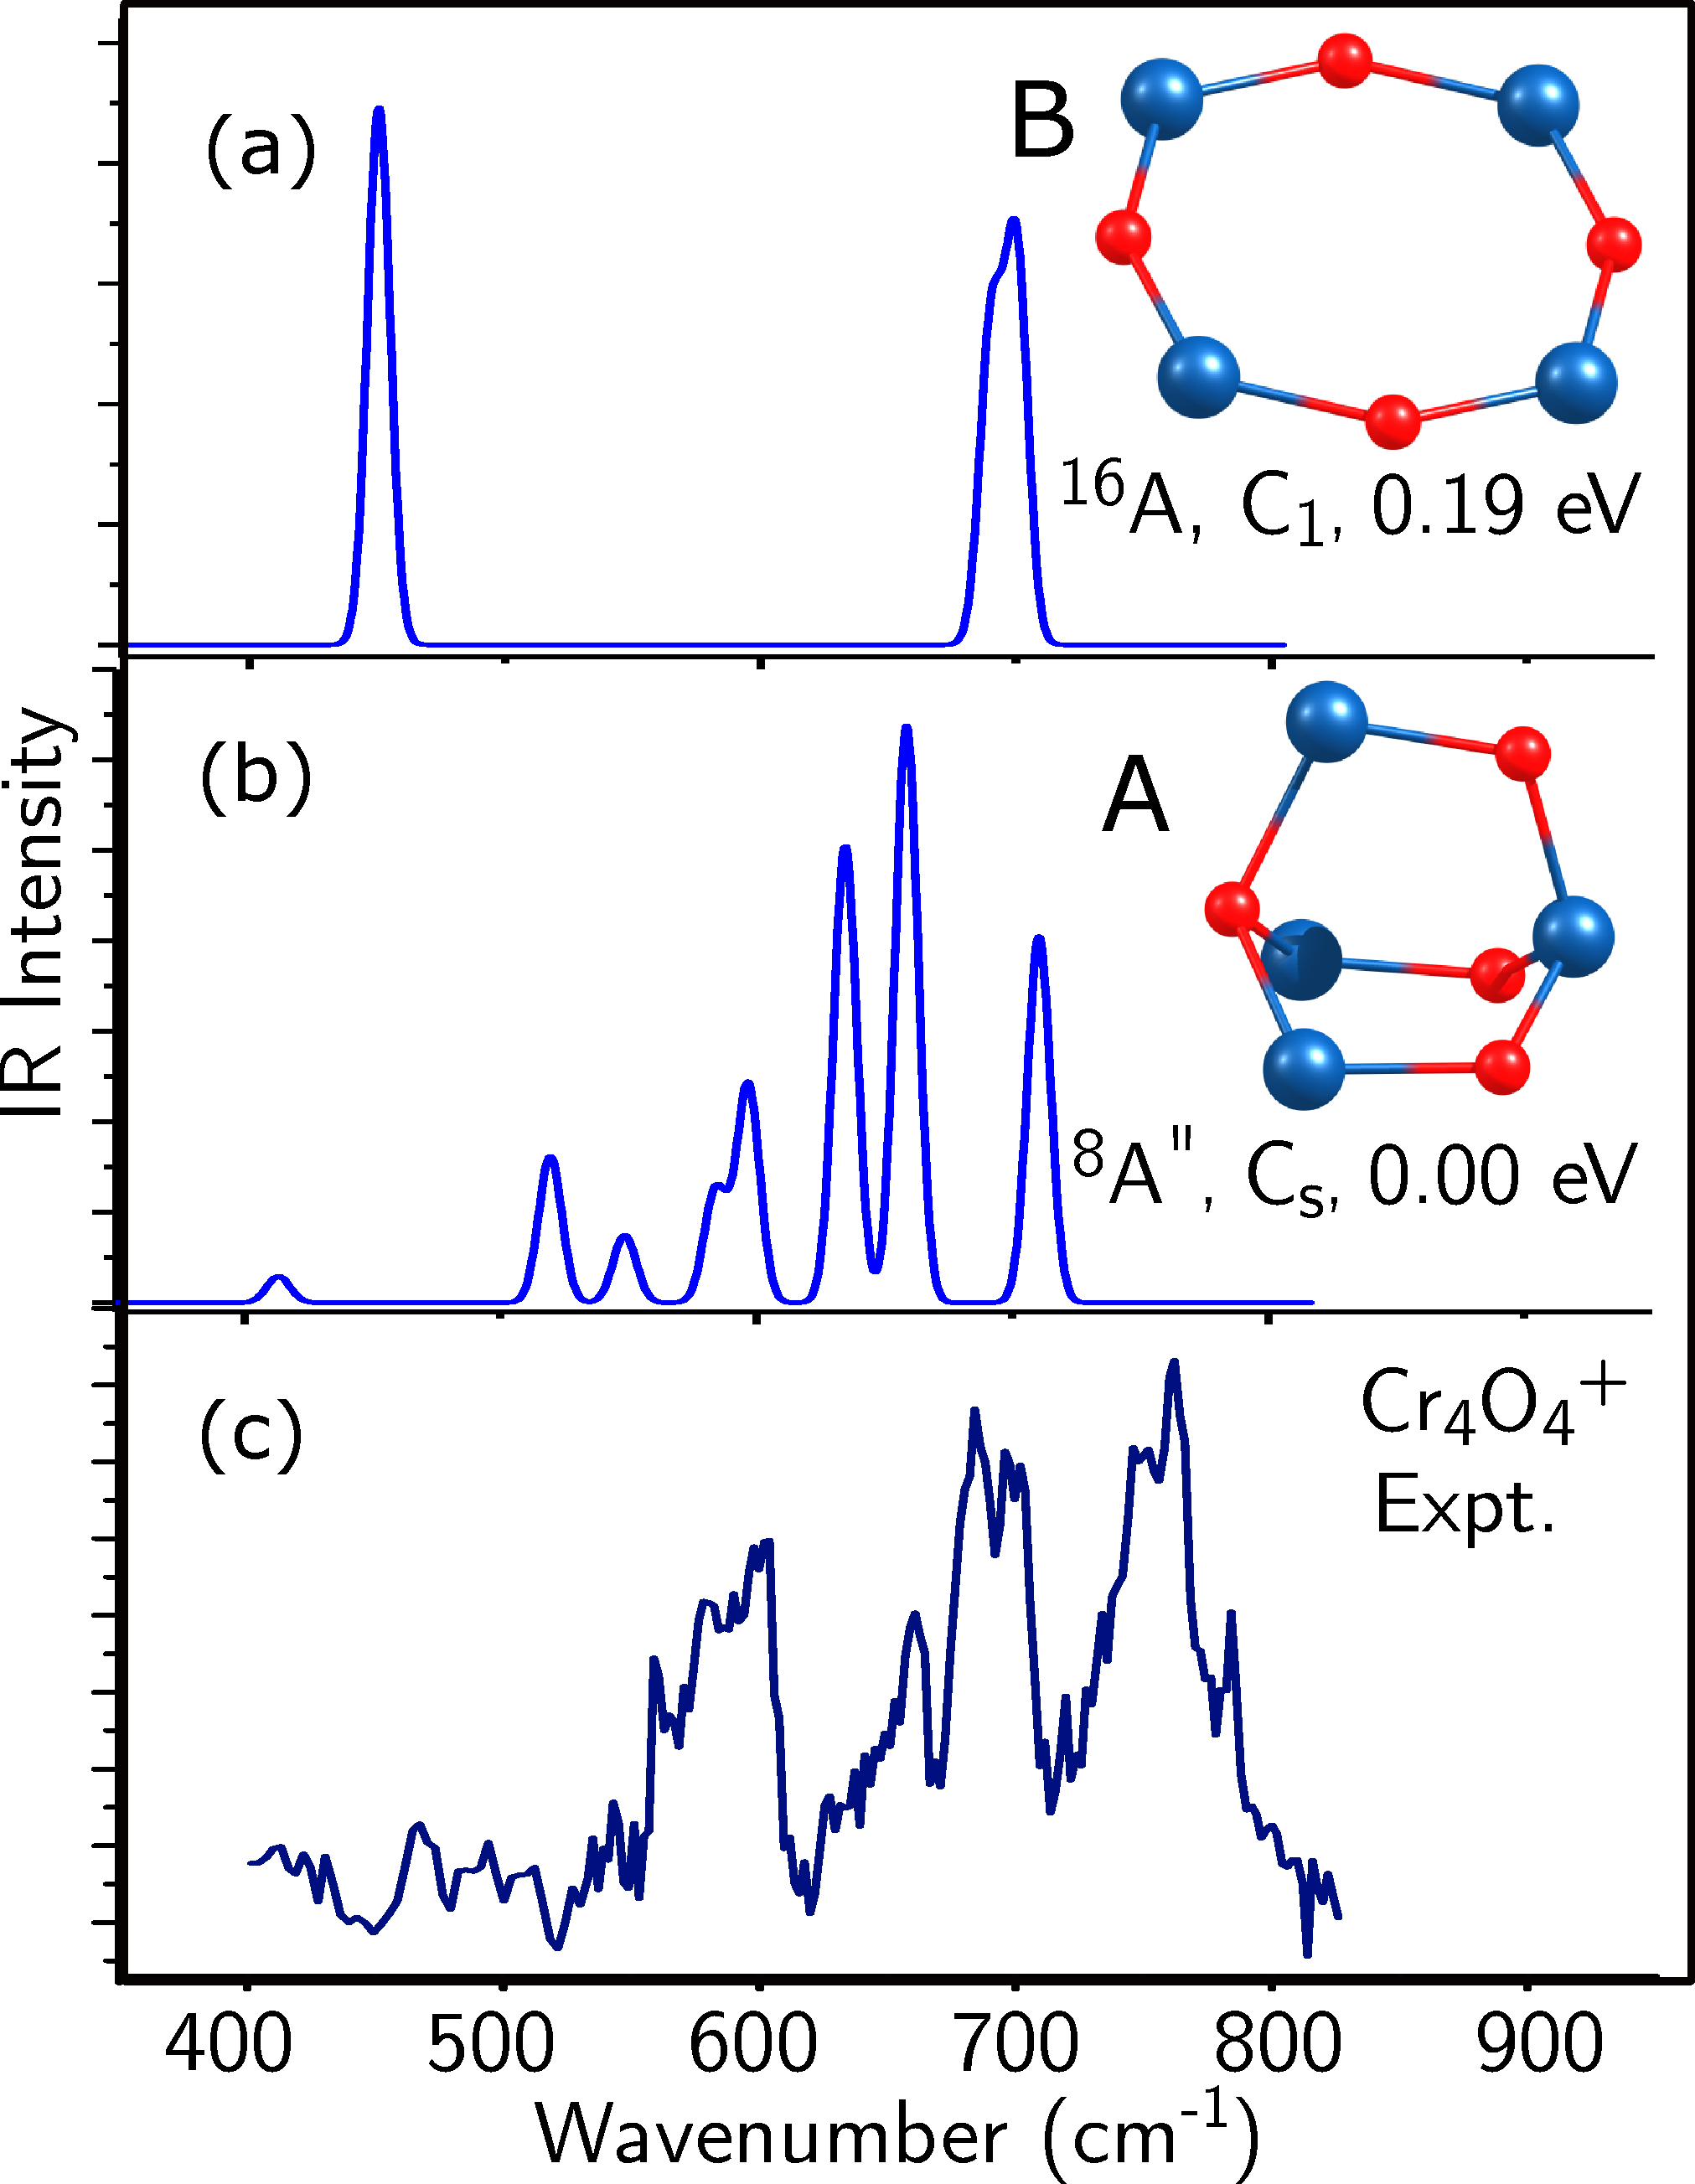
\includegraphics[width=0.45\textwidth]{Cr4O4}
	\caption{Experimental \acrshort{irpd} spectra and simulated harmonic \acrshort{ir} spectra of \ch{Cr4O4+}. The geometries of the two most stable isomers are shown as insets.}
	\label{fig:Cr4O4}
\end{figure}



From the above results, one can recognize that different structural motifs result in different \acrshort{ir} spectra. In certain cases also similar structural motifs with a different spin state and thus different magnetic configurations can be distinguished by their \acrshort{ir} spectra. This is the case for \ch{Cr4O4+}. Figure \ref{fig:spin-spec} presents four different spin configurations (quartet, sextet, octet, and dectet) of structural isomer A of \ch{Cr4O4+}, with the octet spin state having the lowest energy. The simulated \acrshort{ir} spectra of those different spin states are distinct from each other. This implies that the \acrshort{irpd} technique is, in this specific case, a suitable tool to not only probe the geometric structure but also spin configurations. This constitutes clear evidence of the direct relationship between the identification of vibrational spectra with the \acrshort{irpd} technique and magnetic properties.  


\begin{figure}[htb!]
	\centering
	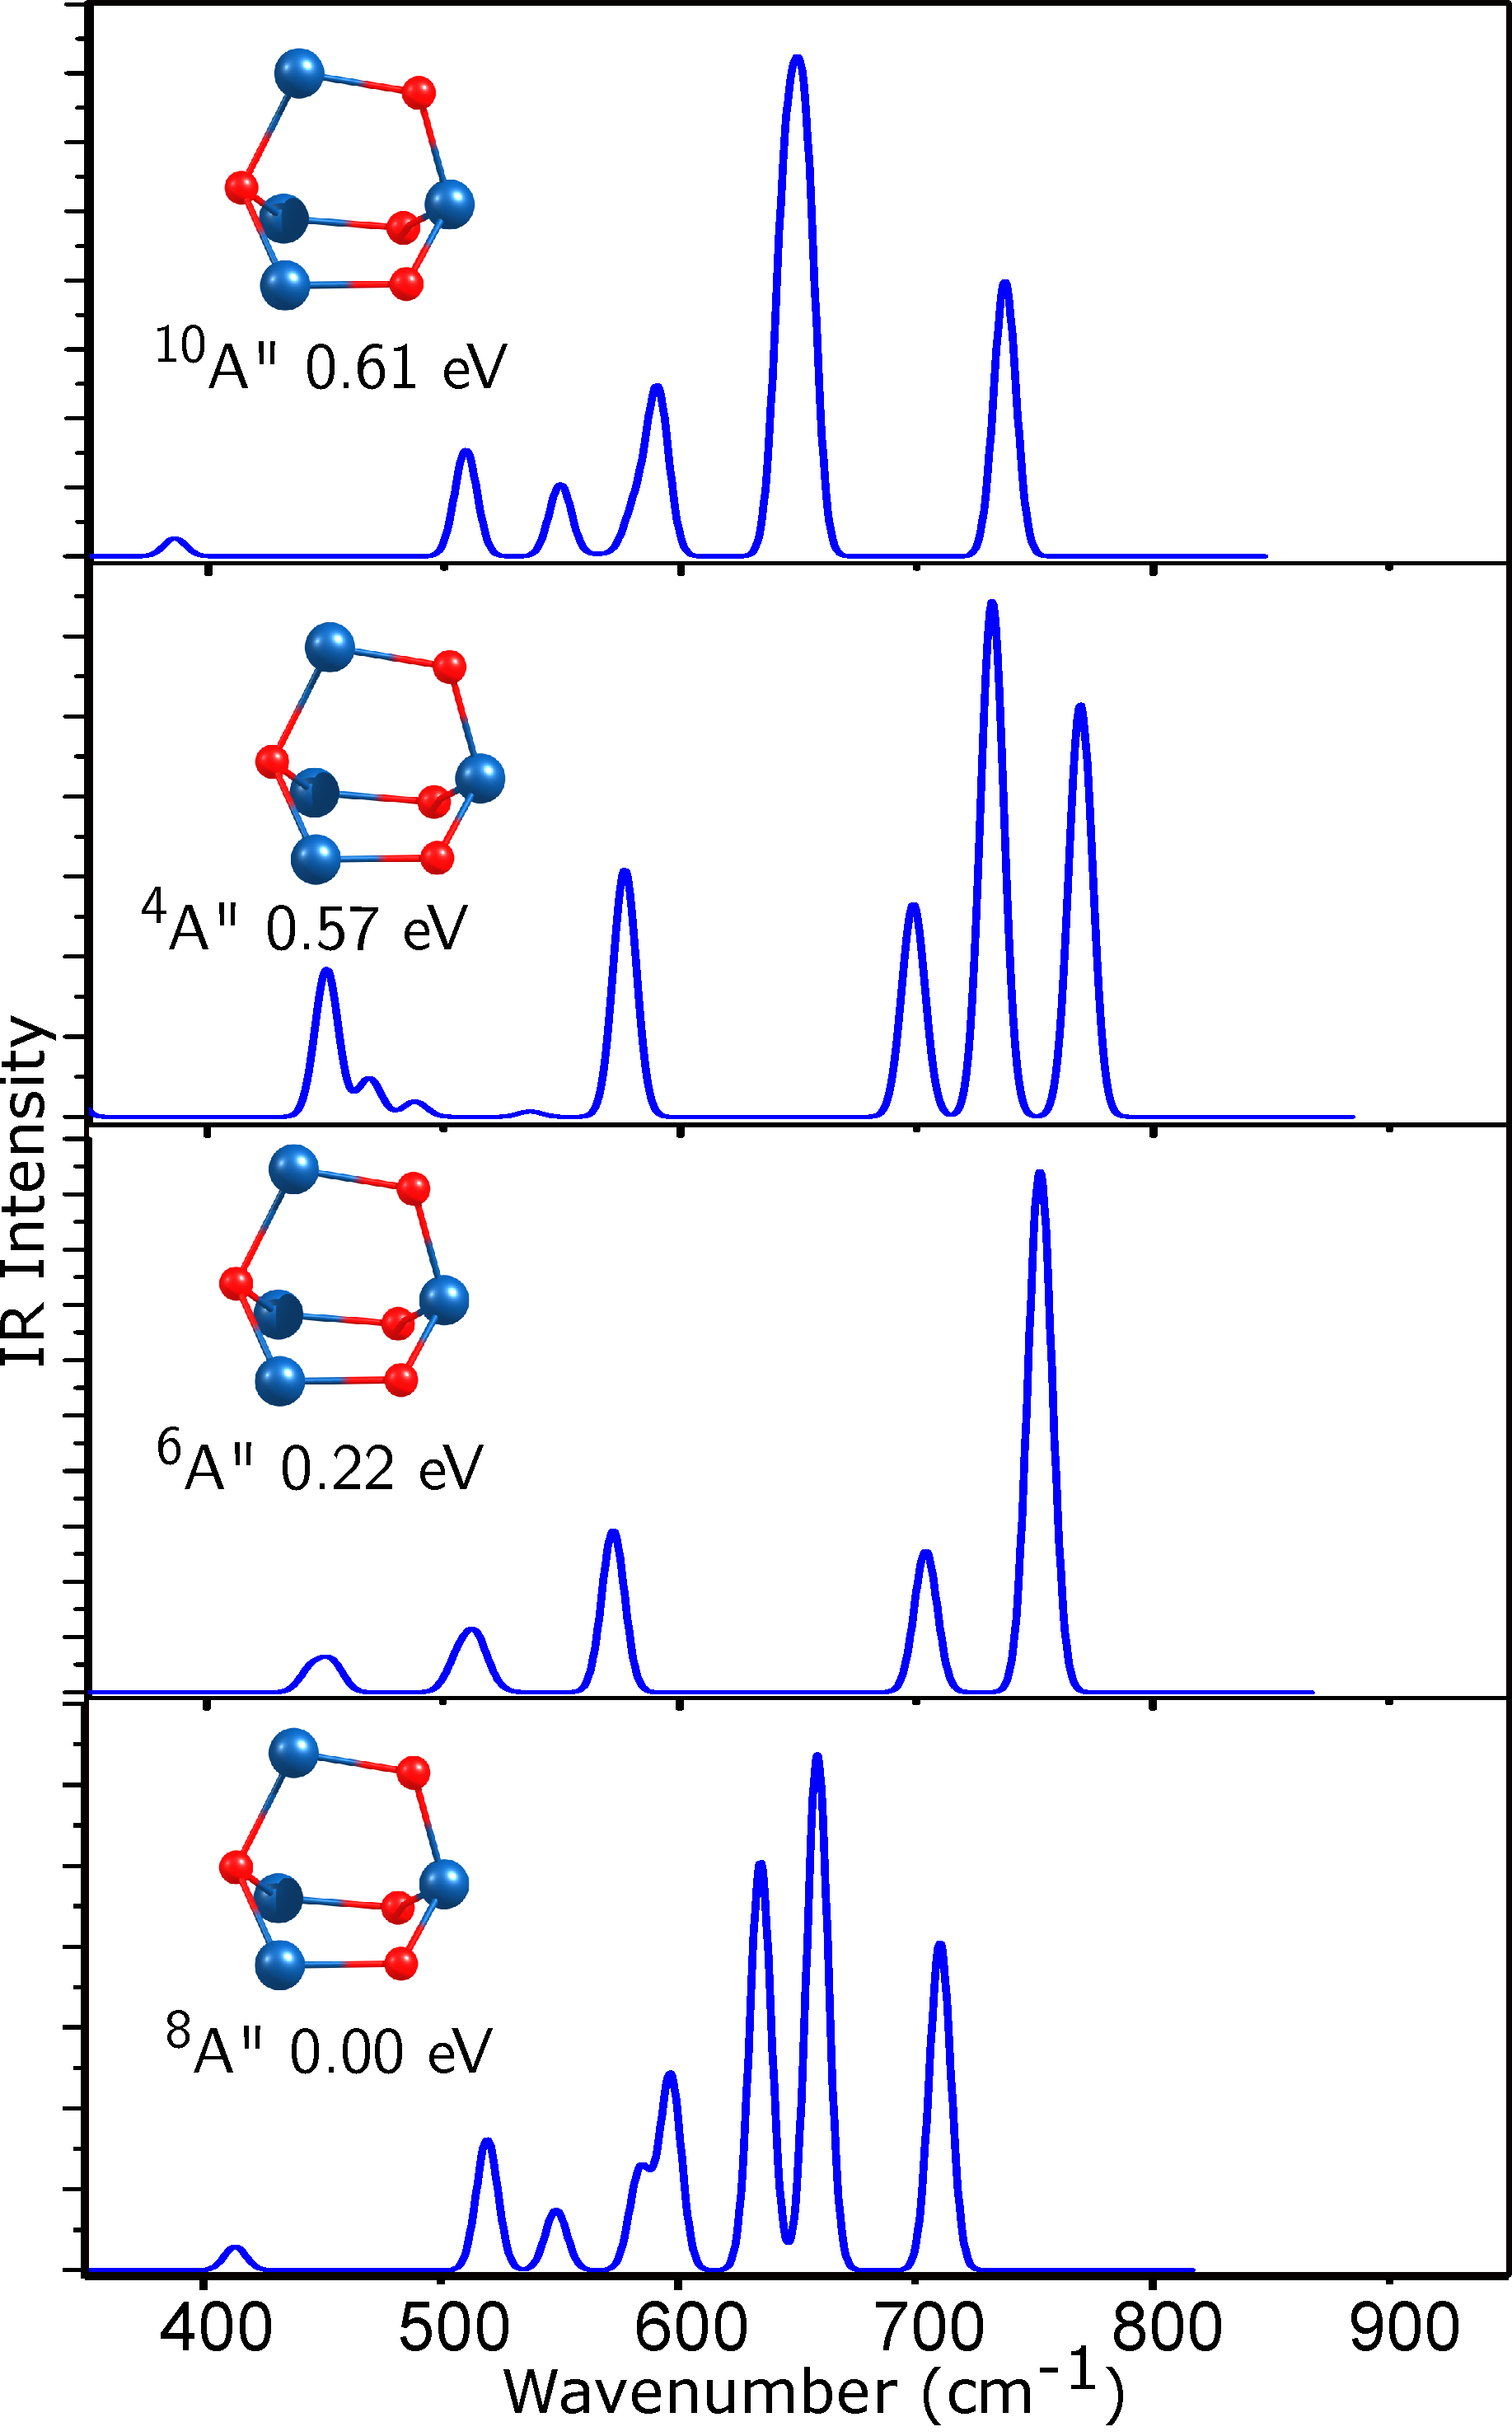
\includegraphics[width=0.45\textwidth]{Cr4O4-spin-spec}
	\caption{Simulated harmonic \acrshort{ir} spectra of structural isomer A of \ch{Cr4O4+} in four different spin states.}
	\label{fig:spin-spec}
\end{figure}




%%%%%%%%%%%%%%%%%%%%%%%%
\subsection{Magnetic Properties} 
%%%%%%%%%%%%%%%%%%%%%%%%

After assigning the geometric structures and the electronic states of the chromium oxide clusters by comparing the measured with simulated \acrshort{ir} spectra, computations can be used to analyze the magnetic properties of the clusters. Local spin moments of individual atoms, which combine to give total spin magnetic moments of clusters, are graphically presented in Figure \ref{fig:magnet}. Values of these local spin magnetic moments are given in Table \ref{table:magnetic}. Also \ch{Cr3+}, \ch{Cr3O4+} and \ch{Cr3O5+} are added to the figure and the table. For these sizes, we only have computational results and no assignment of their structure based on the infrared spectra was performed. The spin magnetic configurations of the clusters can be divided into two groups: (i) clusters in which chromium spin moments are ferromagnetically coupled (\ch{Cr2O2+}, \ch{Cr3O3+}, \ch{Cr3O4+}, and \ch{Cr3O5+}) and (ii) clusters in which metallic spin moments are ferrimagnetically coupled (\ch{Cr3+}, \ch{Cr3O+}, \ch{Cr3O2+}, and \ch{Cr4O4+}). In the ground-state structures of \ch{Cr2O2+}, \ch{Cr3O3+}, \ch{Cr3O4+}, and \ch{Cr3O5+} all spin magnetic moments of the chromium atoms are parallel, which leads to high values of 7, 11, 9, and 7 $\mu_B$, respectively. In \ch{Cr3+}, \ch{Cr3O+}, \ch{Cr3O2+} and \ch{Cr4O4+} the total spin magnetic moment is reduced compared to the maximal values, resulting in spin moments of 3, 5, 5 and 7 $\mu_B$, respectively. 

\begin{figure}[htb!]
	\centering
	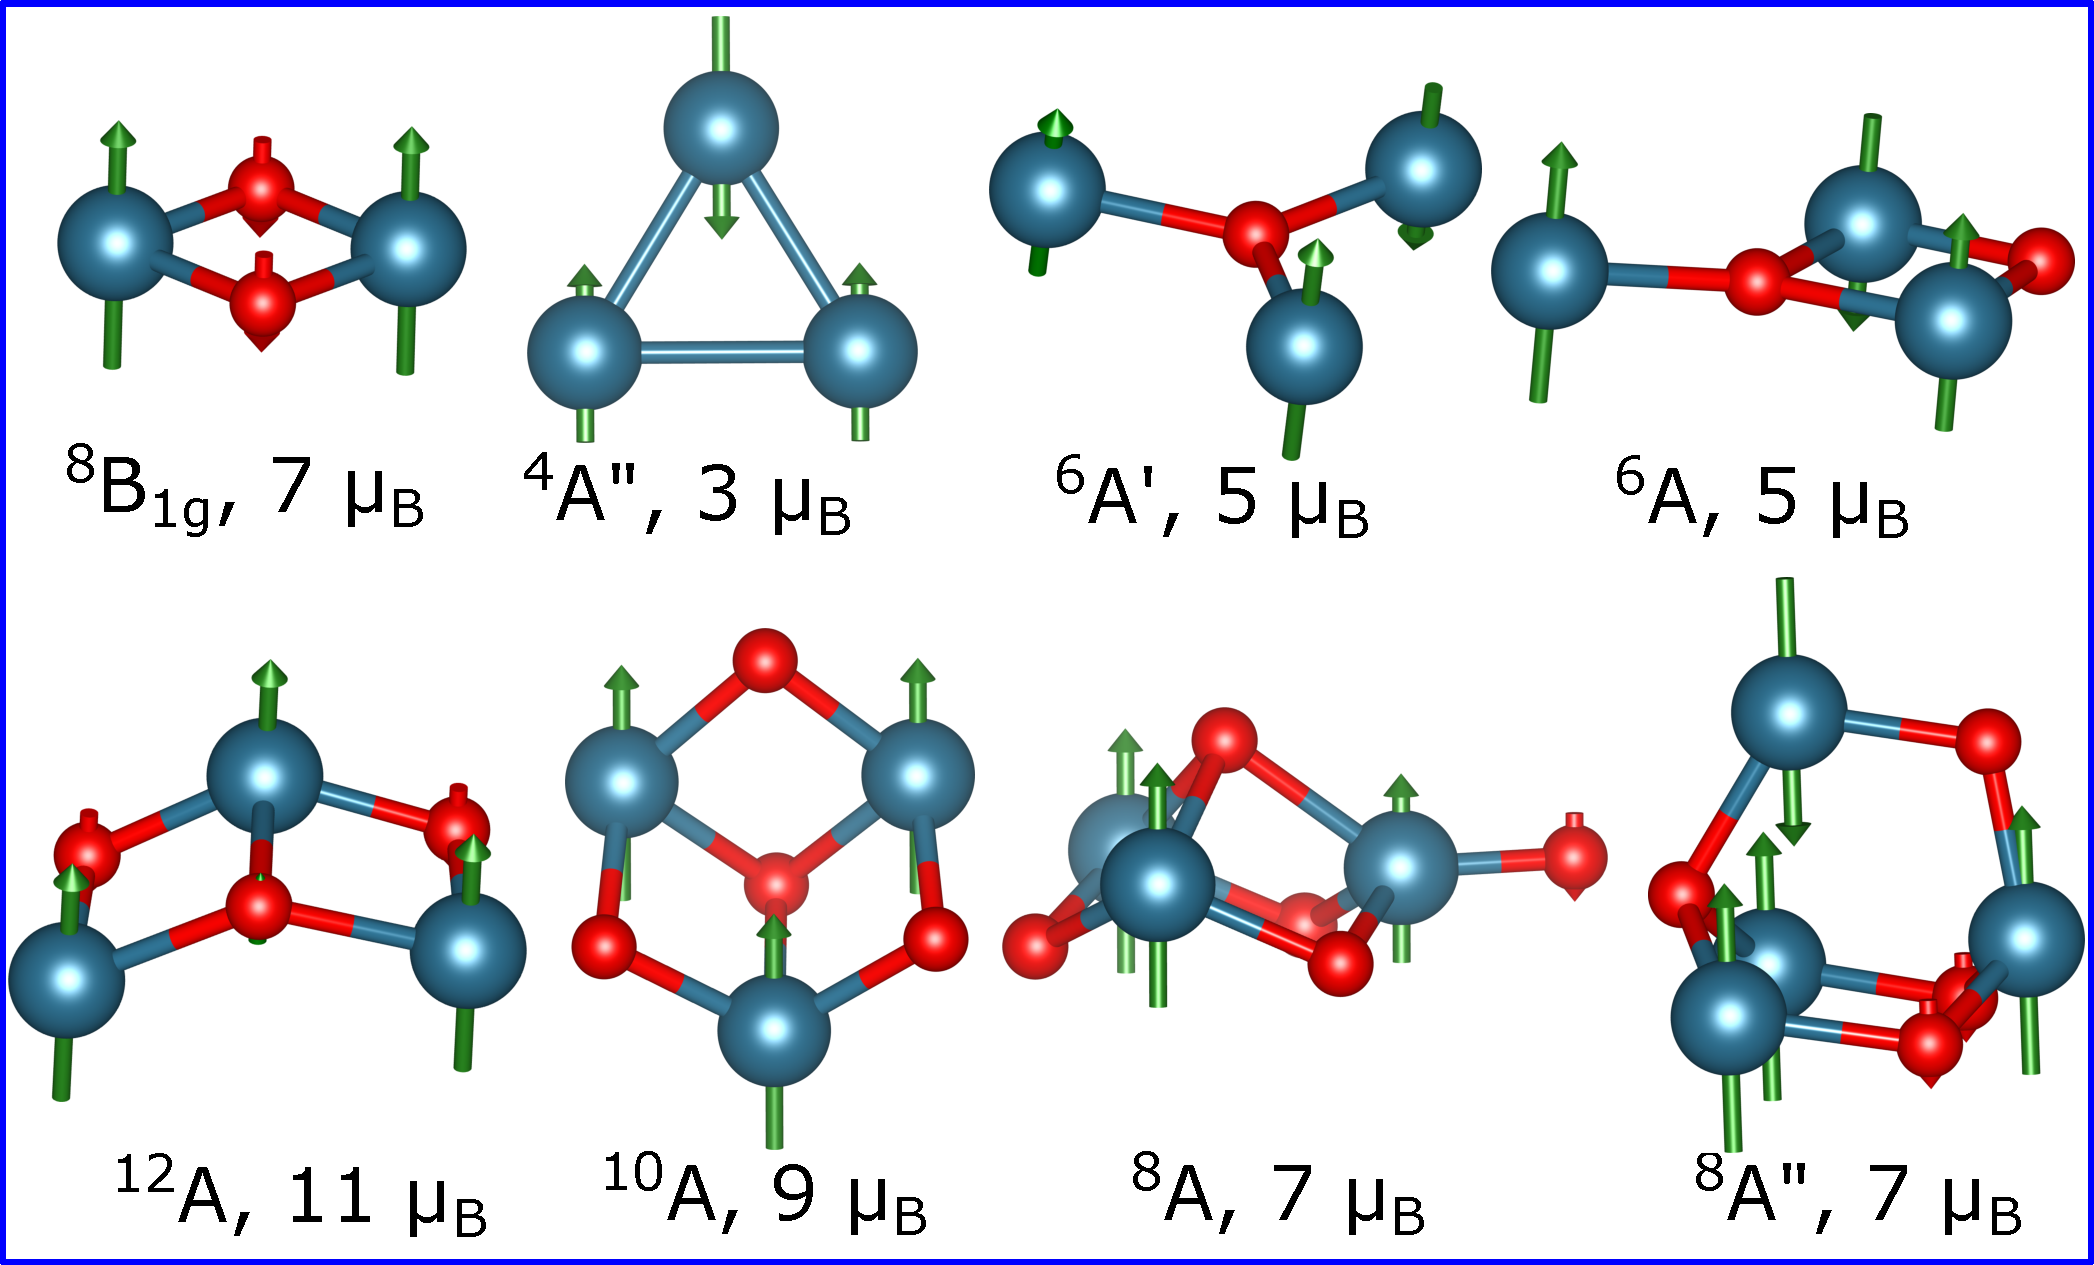
\includegraphics[scale=0.18]{magnet-moment}
	\caption{Structures of \ch{Cr2O2+}, \ch{Cr3O+}, \ch{Cr3O2+}, \ch{Cr3O3+}, and \ch{Cr4O4+} as assigned by comparison of simulated \acrshort{ir} spectra with the experimental \acrshort{irpd} spectra. In addition, the structures of \ch{Cr3+}, \ch{Cr3O4+} and \ch{Cr3O5+}, for which no \acrshort{irpd} data is available, are added to the figure. Spin magnetic moments of \ch{Cr3+}, \ch{Cr3O4+} and \ch{Cr3O5+} were calculated from their energetically lowest geometry and electronic states. Chromium and oxygen atoms are represented by blue and red balls, respectively. Green (red) arrows indicate the orientation of the local spin magnetic moments (> 0.05 $\mu_B$) on the chromium (oxygen) atoms.}
	\label{fig:magnet}
\end{figure}


\begin{landscape}
\begin{table}[htb!]
	\centering
	\begin{threeparttable}
	\caption{Total Spin Magnetic Moments of Clusters and Local Spin Magnetic Moments of Chromium and Oxygen Atoms\tnote{(a)}}
	\label{table:magnetic}
	\begin{tabular}{llcrrrrrrrrr}
		\hline
		\multirow{2}{*}{cluster} & \multirow{2}{*}{state} & \multirow{2}{*}{\begin{tabular}[c]{@{}l@{}}spin magnetic\\  moment ($\mu_B$)\end{tabular}} & \multicolumn{9}{c}{local spin magnetic moment ($\mu_B$)}   \\ \cline{4-12} 
					  &        			&      & Cr$_1$& Cr$_2$& Cr$_3$& Cr$_4$& O$_1$ & O$_2$ &  O$_3$ & O$_4$ & O$_5$		\\ \hline
		Cr$_2$O$_2^+$ & $^8$B$_{1g}$   	& 7    & +3.6 & +3.6 &       &       & -0.07 & -0.07 &        &       &			\\
		Cr$_3^+$	  & $^4$A 			& 3	   & -4.5 & +3.8 & +3.8 &	   &	   &	   &	    &	    &			\\
		Cr$_3$O$^+$   & $^6$A$'$    	& 5    & +4.6 & -4.5 & +4.9 &       & -0.02 &       &        &       &			\\
		Cr$_3$O$_2^+$ & $^6$A    		& 5    & +4.9 & +3.9 & -3.7 &       & -0.03 &  0.00 &        &       &			\\
		Cr$_3$O$_3^+$ & $^{12}$A    	& 11   & +3.1 & +4.0 & +4.0 &       & -0.06 & -0.06 & +0.01  &       &			\\
		Cr$_3$O$_4^+$ & $^{10}$A 		& 9	   & +3.0 & +3.0 & +3.0 &	   & -0.02 & -0.02 & -0.02  & +0.06 &			\\	
		Cr$_3$O$_5^+$ & $^8$A 			& 7	   & +1.3 & +2.9 & +2.9 &	   & -0.12 & -0.01 & +0.02  & +0.02 & +0.05	    \\
		Cr$_4$O$_4^+$ & $^8$A$"$    	& 7    & +3.8 & -3.1 & +3.8 & +2.6 & -0.08 & -0.01 & -0.08  & +0.03 &			 \\ \hline
	\end{tabular}
	\begin{tablenotes}
		\item[(a)] All values were calculated making use of natural bond orbital (NBO) analysis on the basis of the TPSS electron density.
	\end{tablenotes}
	\end{threeparttable}
	\end{table}
\end{landscape}

%%%% Interaction in 

3\textit{d}-3\textit{d} bonding-formation and superexchange-type interactions were demonstrated to underlie the corresponding magnetic properties in pure chromium clusters (\ch{Cr2^{0}}, \ch{Cr3^{+/0}}) \cite{bondybey1983, Cr2t, Cr2x} and dichromium oxide clusters (\ch{Cr2O2^{-/0}}, and \ch{Cr2O3^{-/0}}).\cite{Tono2003, Tono2003B, paul2009Cr2On} In this work, we find small antiferromagnetic spin moments on the oxygen atoms in \ch{Cr2O2+} and \ch{Cr3O3+}. Coupling between the chromium and oxygen sites in these clusters occurs through the hybridization between Cr 3\textit{d} and O 2\textit{p} orbitals. Such an orbital interaction is known as superexchange, and it enhances the parallel spin coupling between chromium atoms. \cite{Tono2003,Tono2003B,paul2009Cr2On} Figure \ref{fig:dos} pictorially provides the total density of states (\acrshort{tdos}) and partial density of states (\acrshort{pdos}) of \ch{Cr3O3+} and \ch{Cr3O+}. In the case of \ch{Cr3O3+}, the \acrshort{pdos} (Figure \ref{fig:dos}c) reveals, particularly for the alpha occupied orbitals, strong hybridization between the chromium 3\textit{d} and the oxygen 2p orbitals in the -15.0 to -9.0 eV range (-9.0 eV is the energy of the \acrshort{homo}). The \ch{Cr3+}, \ch{Cr3O+}, \ch{Cr3O2+}, and \ch{Cr4O4+} clusters disclose ferrimagnetic magnetic behavior, in which one of chromium atoms has its magnetic moment in the reverse direction of the others. By analyzing interaction between the two closest chromium atoms in the \ch{C_s} isomer of \ch{Cr3O+}, bonding-like features are found between those two chromium atoms (see Figure \href{https://pubs.acs.org/doi/suppl/10.1021/acs.jpcc.8b10035/suppl_file/jp8b10035_si_002.pdf}{\textcolor{blue}{S14}}). The 3\textit{d} \acrshort{pdos} of the antiferromagnetically coupled chromium atoms of this cluster show energetic overlap between $\alpha$ and $\beta$ 3\textit{d} occupied orbitals in the -10 to -8.5 eV range (Figure \ref{fig:dos}d). Therefore, 3\textit{d}-3\textit{d}-like bonding between two closest chromium atoms causes an antiferromagnetic coupling of the local spin magnetic moments, similar as in the \ch{Cr2} dimers. \cite{Cr2t,Cr2x} A similar bonding-type formation is believed to be present in \ch{Cr3O2+} and \ch{Cr4O4+} (see Figures \href{https://pubs.acs.org/doi/suppl/10.1021/acs.jpcc.8b10035/suppl_file/jp8b10035_si_002.pdf}{\textcolor{blue}{S14}} and \href{https://pubs.acs.org/doi/suppl/10.1021/acs.jpcc.8b10035/suppl_file/jp8b10035_si_002.pdf}{\textcolor{blue}{S15}}), where the spin moment of one of the chromium atoms in antiparallel to the other ones. 


\begin{figure}[htb!]
	\centering
	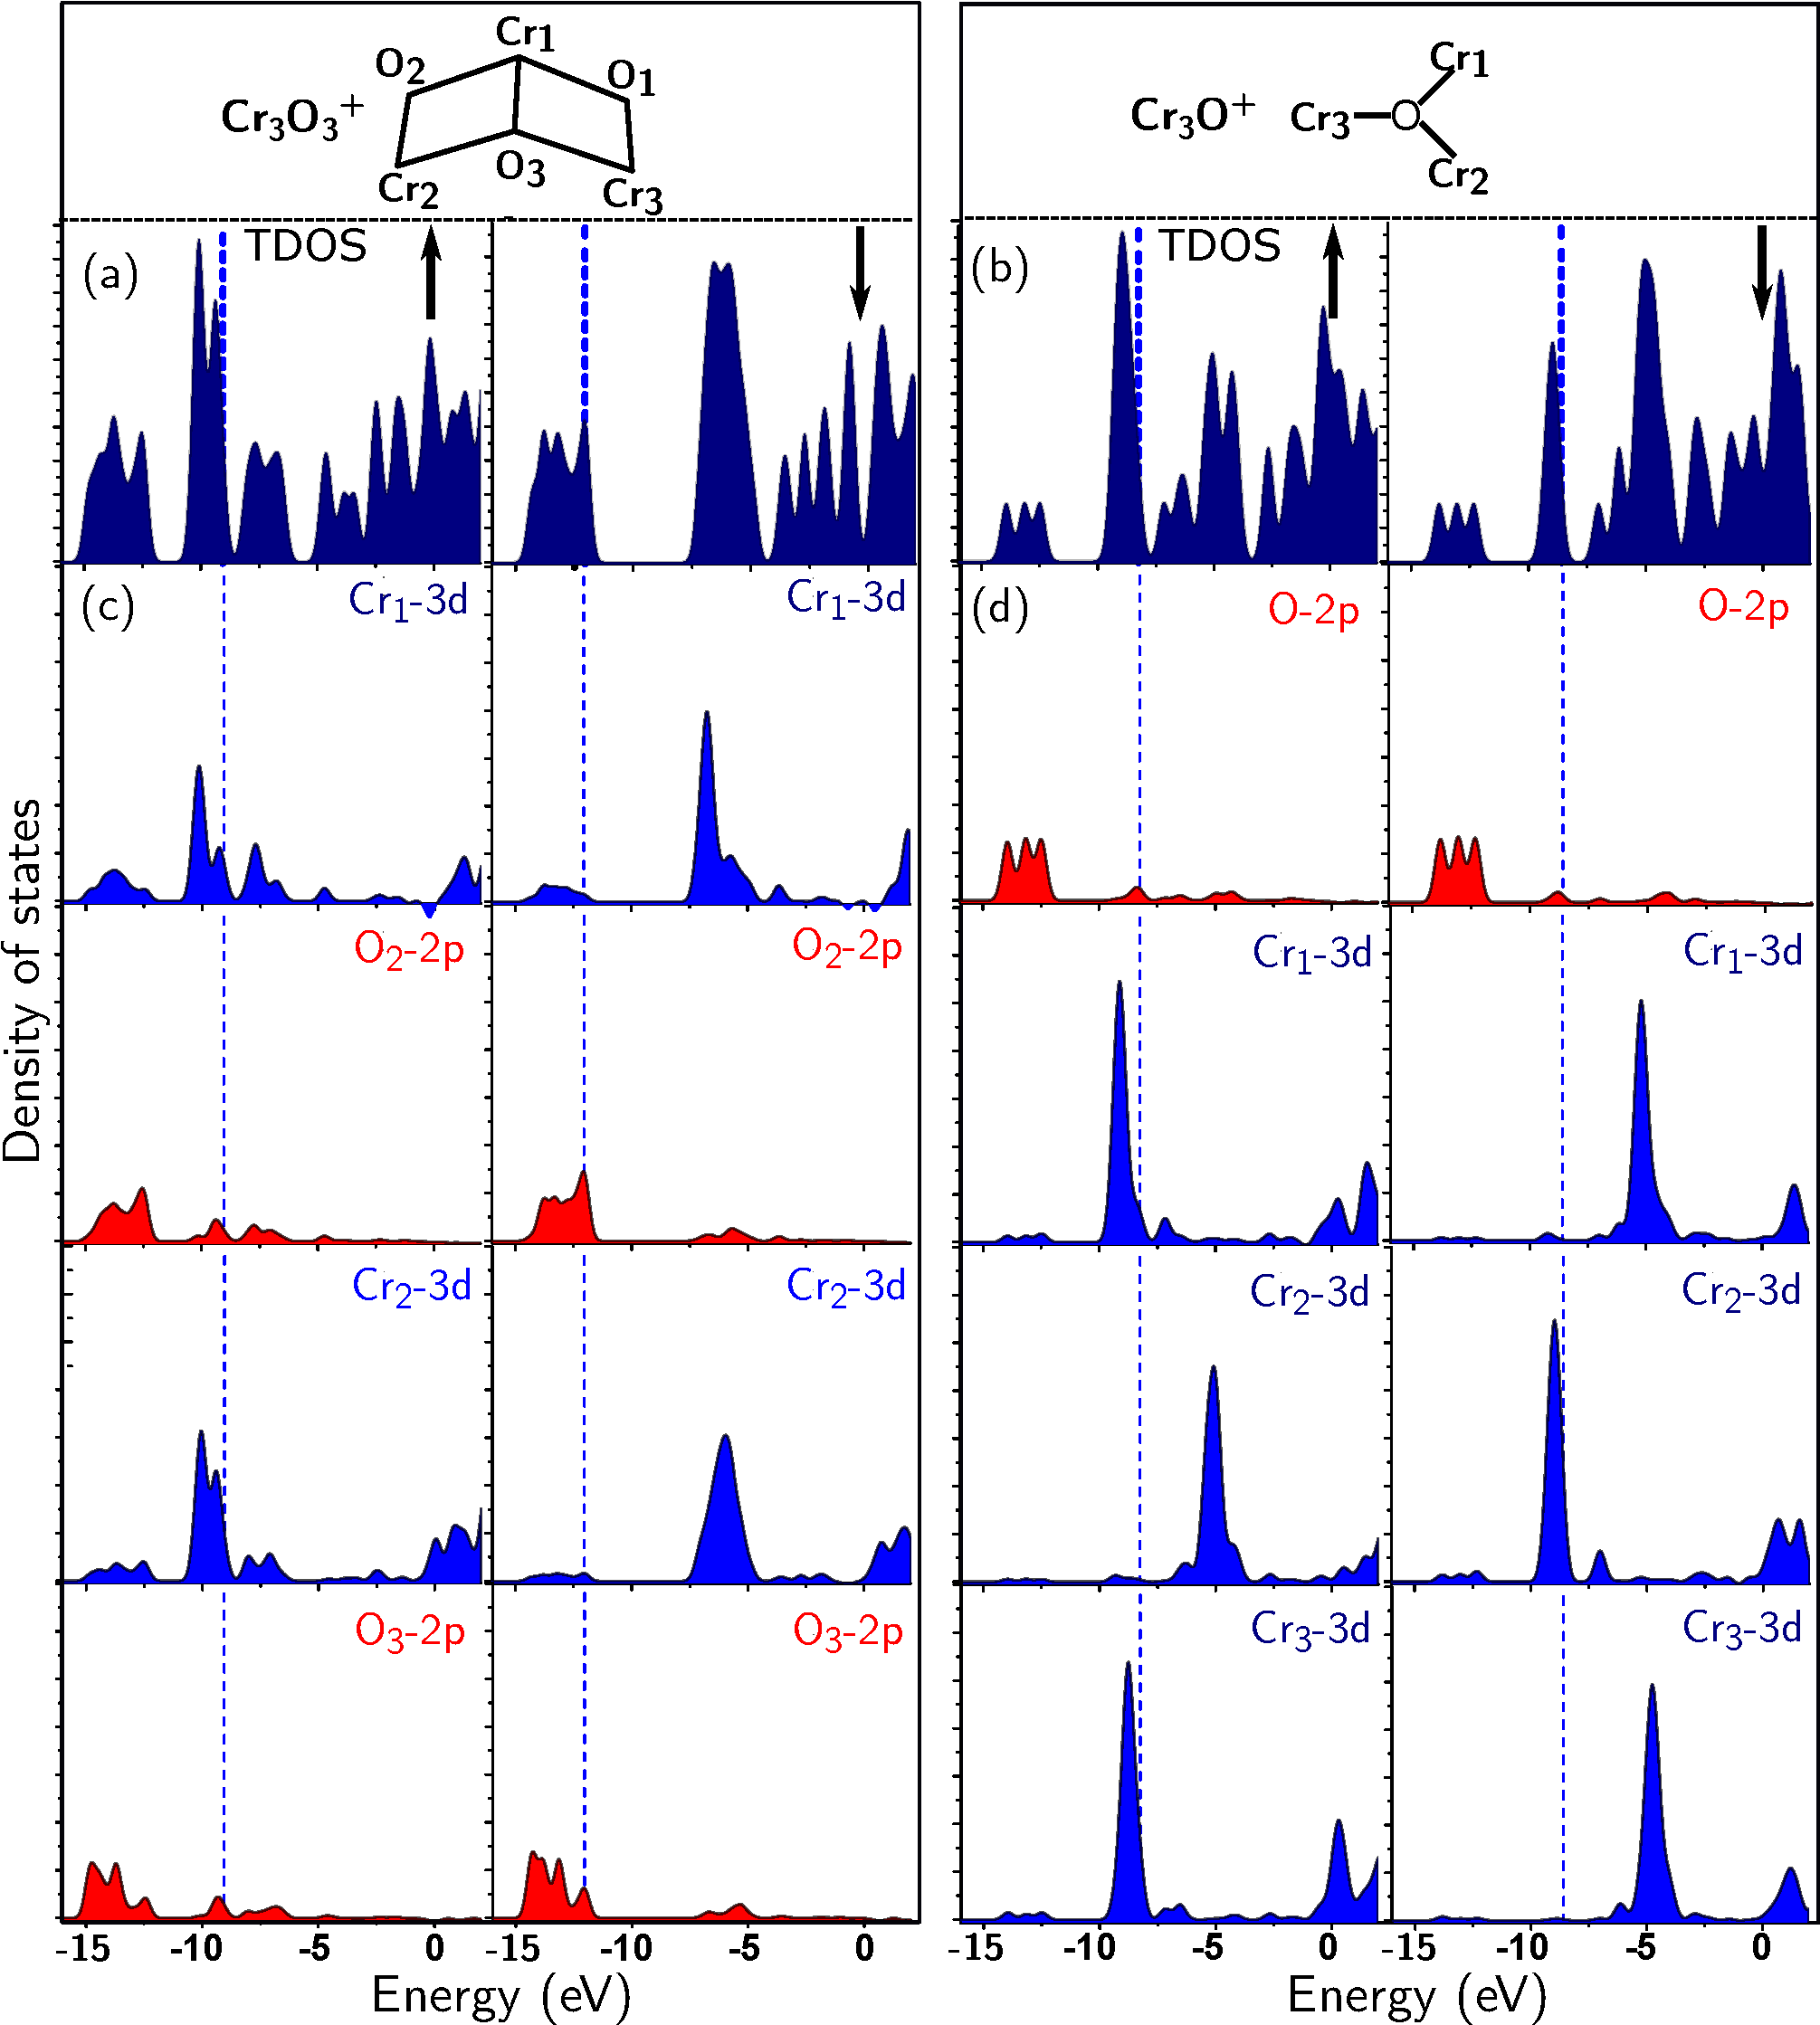
\includegraphics[width=\textwidth]{DOS.pdf}
	\caption{Total density of states (\acrshort{tdos}) and partial density of states (\acrshort{pdos}) of \ch{Cr3O3+} (left part) and \ch{Cr3O+} (right part). For each part the left (right) side corresponds to alpha or up (beta or down) orbitals as indicated by the black arrows: (a) \acrshort{tdos} of \ch{Cr3O3+}, (b) \acrshort{tdos} of \ch{Cr3O+}, (c) \acrshort{pdos} of \ch{Cr3O3+}, and (d) \acrshort{pdos} of \ch{Cr3O+}. For \acrshort{pdos}, the projections in oxygen-2p (chromium-3\textit{d}) orbitals are shown in red (blue). Atoms are numbered according to the structures shown in the insets. Vertical short dashed lines indicate the highest occupied alpha and beta orbitals.} 
	\label{fig:dos}
\end{figure}



Next, we investigate the effect of atom-by-atom oxygen addition to the geometry and magnetism of the \ch{Cr3+} metallic cluster. Figure \ref{fig:magevo} presents the magnetic evolution of \ch{Cr3O_n+} (n = 0 -- 5). With the addition of oxygen atoms, the total magnetic moment increases from n = 0 (3 $\mu_B$) to n = 3 (11 $\mu_B$). Such a strong increase of the total magnetic moment implies that direct 3\textit{d}-3\textit{d} bonding-type interaction, which favors antiferromagnetic coupling, becomes weaker upon addition of oxygen atoms, reducing the 3\textit{d}-3\textit{d} interaction. The 3\textit{d}-3\textit{d} bonding-type formation is dominated by the superexchange interaction in \ch{Cr3O3+}, leading to a high total spin magnetic moment (11 $\mu_B$). The total spin magnetic moment is gradually reduced if more oxygen atoms are added (n = 4 and n = 5). Finally, the magnetic moment is expected to be quenched, as was computationally found for the di-chromium oxides \ch{Cr2O_n} \cite{GutsevCr2On} (n $\geq$ 6). This result unravels how the oxygen concentration affects and controls the total magnetic properties of trichromium oxides.


\begin{figure}[htb!]
	\centering
	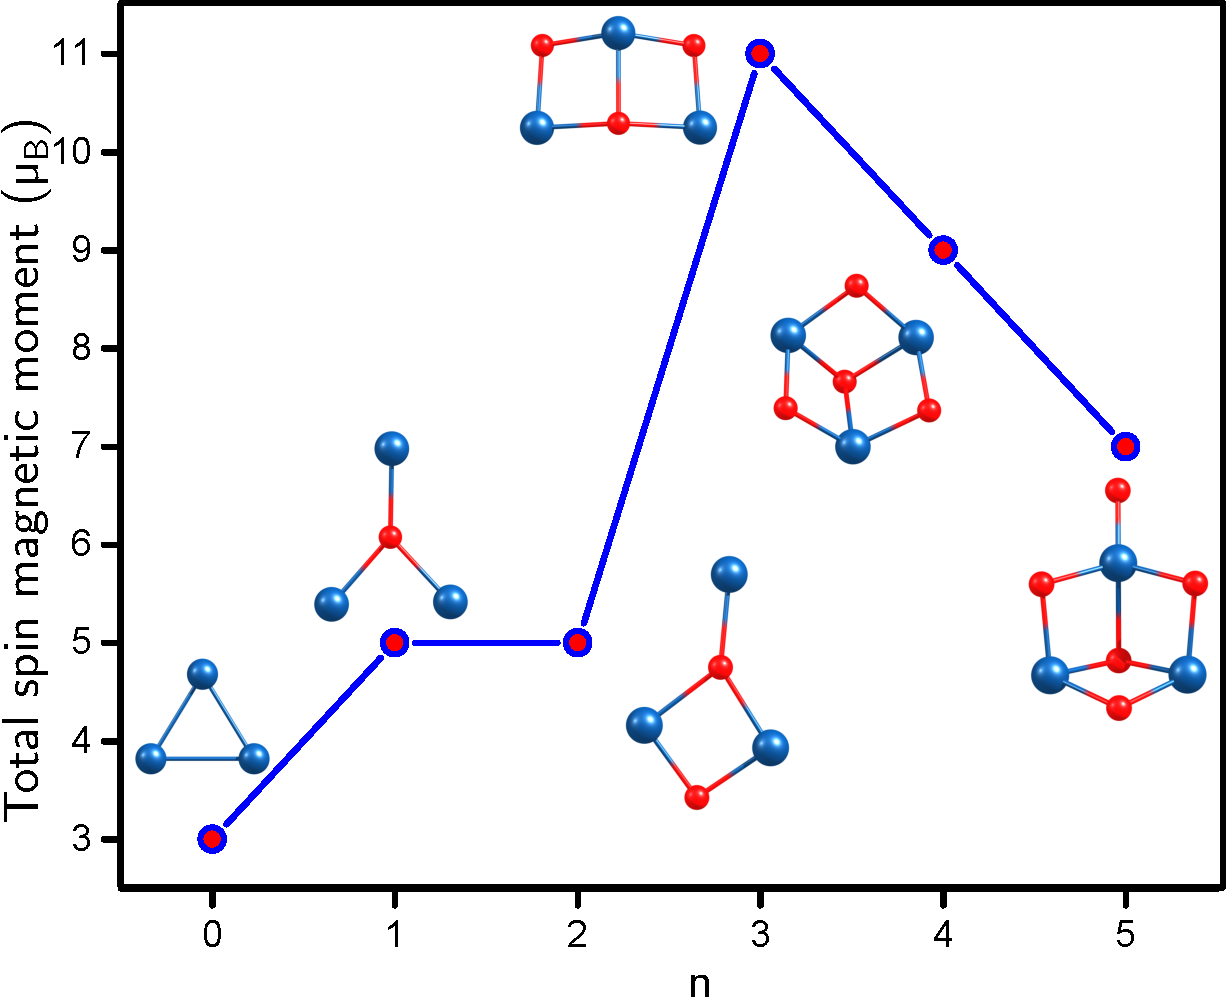
\includegraphics[scale=0.4]{magm-evo}
	\caption{Evolution of the total spin magnetic moment for \ch{Cr3O_n^+} (n = 0 -- 5) clusters.} 
	\label{fig:magevo}
\end{figure}




Overall the evolution of the structures and the magnetic configurations with the oxygen concentration indicates that the highest magnetic moments, i.e. parallel alignment of the local Cr spin magnetic moments, are obtained in suboxides that have enough oxygen atoms to form \ch{Cr-O-Cr} bridges with a unique O atom between each pair of Cr atoms. For \ch{Cr3O_n+} this occurs in \ch{Cr3O3+}. In this cluster the superexchange interaction is maximized and occurs without strong reduction of the local magnetic moments on the involved Cr atom (see Table \ref{table:magnetic}). Addition of more oxygen atoms (i.e. in \ch{Cr3O4+} and \ch{Cr3O5+}) results in the formation of \ch{Cr-O} bonds with individual Cr atoms and the delocalization of the Cr 3\textit{d} electrons in \ch{Cr-O} shared orbitals. Such capturing of unpaired Cr 3\textit{d} electrons reduces the Cr local magnetic moments. The observation of this magnetic configuration dependence on the oxygen concentration is empirical. An in-debt explanation may be the subject of follow-up studies.




\section{Conclusion}

In conclusion, several cationic chromium-rich oxides were synthesized and characterized through \acrshort{ir} spectral characteristics. The magnetic states of these clusters were studied to reveal insights into their magnetic properties. Oxygen plays an important role in controlling the magnetic configurations. Superexchange interaction through oxygen bridging sites causes ferromagnetic coupling of the chromium atoms in \ch{Cr2O2+} and \ch{Cr3O3+}. The ferrimagnetic behavior of \ch{Cr3O+}, \ch{Cr3O2+}, and \ch{Cr4O4+} is attributed to the bonds between the metal atoms, in which 3\textit{d} orbitals of nearby chromium atoms directly interact with each other resulting in lower total spin magnetic moments. This study indicates that the highest possible total magnetic moments are obtained in suboxides with a comparable number of oxygen and chromium atoms that have a unique oxygen atom in a single \ch{Cr-O-Cr} bridge between each pair of Cr atoms. The addition of more oxygen atoms enhances the delocalization of the Cr 3\textit{d} electrons and reduces the magnetic moment.






%%%%%%%%%%%%%%%%%%%%%%%%%%%%%%%%%%%%%%%%%%%%%%%%%%
% Keep the following \cleardoublepage at the end of this file, 
% otherwise \includeonly includes empty pages.
%\cleardoublepage

\includebibliography
\printbibliography[heading=subbibliography] % print section bibliography

\end{refsection}
